\documentclass[12pt,fleqn]{article}\usepackage{../../common}
\begin{document}
Materyel Mekaniği - 5

Bükülen bir çubuğun formüllerine bir giriş [1] kaynağında yapıldı. Orada
moment-eğri (moment-curvature) formülü gösterilmişti.

$$
M(x) = \frac{E(x)I(x)}{\rho(x)}
\mlabel{1}
$$

Şimdi bu formülü genişletelim, ve bir ikinci derece türeve eşitleyelim.

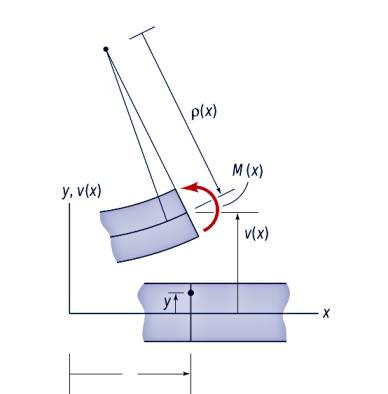
\includegraphics[width=15em]{phy_020_strs_05_01.jpg}

Resimde gösterilen semboller $M$ bükme momenti, $\rho$ çubuğun $+y$ tarafındaki
bükülme çemberinin, eğiminin yarıçapı (radius of curvature).  $v$ ise yine $+y$
kısmındaki yer değişimidir. Çubuğa uygulanan kuvvet dağılımının ne olduğu
önemli değil, sonuçta odaklandığımız çubuğun ufak bir kısmı.

[3] kaynağında bir çemberi (yarıçapını) onun bir eğriye dokunduğu noktadaki
türevler üzerinden temsil etme tekniğini paylaştık. Bu formülü mevcut probleme
uygulayabiliriz.

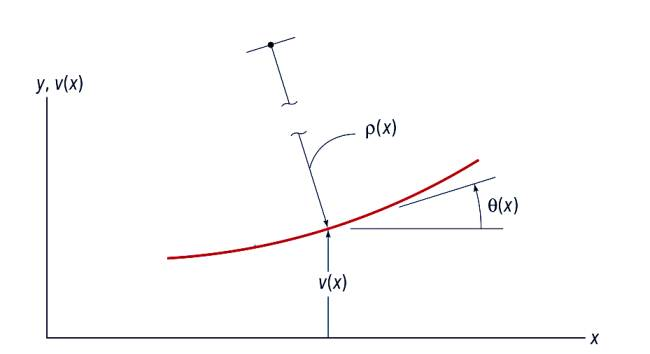
\includegraphics[width=20em]{phy_020_strs_05_02.jpg}

Üstteki örnekte çemberin yarıçapı $\rho$, türevler ise $\ud v / \ud x$.
Formül [2, sf. 466],

$$
\frac{1}{\rho} =
\frac
{\dfrac{\ud^2 v}{\ud x^2}}
{ \left[ 1 + \left( \dfrac{\ud v}{\ud x}  \right)^2 \right]^{3/2} }
$$

Üstteki problemde eğim çok ufaktır o zaman $\ud v / \ud x$ ufak kabul edilir
(resimdeki eğim eğitim amaçlı abartılmış), demek ki bölendeki kare hesabı
daha da ufalır, geriye sadece 1 kalır, 1 ile bölümü yok sayarız, geriye kalanlar

$$
\frac{1}{\rho} \approx \frac{\ud^2 v}{\ud x^2}
\mlabel{2}
$$

Şimdi (1) formülünü tekrar düzenlersek,

$$
\frac{1}{\rho(x)} = \frac{M(x)}{E(x) I(x)}
$$

diyebilirdik. Bu formülün sol tarafının (2) sol tarafı ile aynı olduğunu
görüyoruz. Demek ki onları eşitleyebiliriz, moment-eğri formülü şu hale gelir,

$$
\frac{\ud^2 v}{\ud x^2} = \frac{M(x)}{E(x) I(x)}
$$

Formüller daha kısa olsun diye bazı notasyonel ekler yapalım,

$$
v' = \frac{\ud v}{\ud x}, \quad 
v'' = \frac{\ud^2 v}{\ud x^2}, \quad 
M' = \frac{\ud M}{\ud x}, \quad vs..
$$

İki üstteki formül kısa notasyonla söyle olur,

$$
EI v'' = M
\mlabel{3}
$$

Bir formül daha, sonra faydalı olacak, hatırlarsak,

$$
V = \frac{\ud M}{\ud x}
$$

idi, o zaman (3)'teki formülün iki tarafının $x$'e göre türevini alırsak,

$$
EI v''' = \frac{\ud M}{\ud x} = V
$$

Yani [6, sf. 683]

$$
V = EI v''' = EI \frac{\ud^3 v}{\ud x^3}
\mlabel{6}
$$

Problem çözmek için (3)'teki iki dereceli diferansiyel denklemi kullanabiliriz.

Alttaki gibi bir problem olsun,

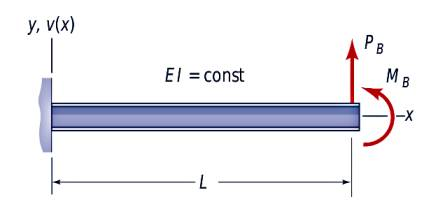
\includegraphics[width=15em]{phy_020_strs_05_03.jpg}

Sol ucu sabit bir dirsekli kiriş (cantilevel beam) var. Bu kirişe dikey yönde en
sağ ucunde $P_B$ yükü ve $M_B$ momenti uygulanıyor. Bu sistemde eğim $v'(x)$ ve
sapma $v(x)$ için gereken ifadeyi bulalım.

Uygulanan iki kuvvet kirişi yukarı doğru eğer, o zaman eğim alttakine benzer,

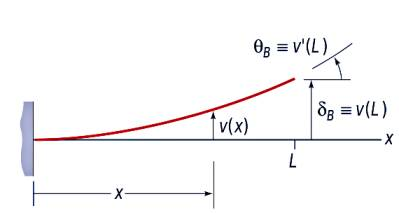
\includegraphics[width=15em]{phy_020_strs_05_04.jpg}

$M(x)$ bulmak için herhangi bir noktadaki hissedilen momentlerin toplamının
sıfır olduğunu hatırlayalım,

$$
M(x) - P_B(L-x) - M_B = 0
$$

Moment-eğri denklemini (3) kullanalım, ve üsttekileri o denkleme koyalım,

$$
EIv'' = M(x) = P_B(L-x) - M_B
$$

Aradığımız sonuç $v$ ve $v'$. O zaman üstteki denklemi iki kere entegre etmemiz
gerekli.

$$
EI v' = M_B x + P_B Lx - P_B \left( \frac{x}{2} \right)^2 + C_1
\mlabel{4}
$$

$$
EIv = M_B \left( \frac{x^2}{2} \right) +
P_B L  \left( \frac{x^2}{2} \right) -
P_B \left( \frac{x^3}{6} \right) +
C_1 x + C_2
\mlabel{5}
$$

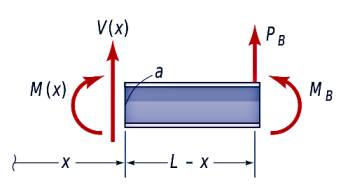
\includegraphics[width=15em]{phy_020_strs_05_05.jpg}

Şimdi sınır şartlarını probleme uygulayalım, bu değerler bilinenler
olarak bilinmeyen değerlerin bulunmasına yardımcı olacak. Sınır şartları
problem tanımında tarif edildi, kirişin bir ucu sabitlenmiş o zaman
$x=0$ noktasında hem eğim hem de sapma sıfır olmalı. Yani

$$
v'(0) = 0,\quad v(0) = 0
$$

Şartlardan ilkini $v'(0)=0$ ve $x=0$ kullanırsak (4) şu hale gelir,

$$
EI v' = C_1 = 0
$$

$v(0)=0$ ve $x=0$ kullanırsak (5) şöyle olur,

$$
EIv = C_2 = 0
$$

Demek ki (4) ve (5) şöyle yazılabilir,

$$
v'(x) = \frac{1}{EI} \left[
  M_B x + P_B Lx - P_B \left( \frac{x}{2} \right)^2
\right]
$$

$$
v(x) = \frac{1}{EI} \left[
  M_B \left( \frac{x^2}{2} \right) + 
  P_B L  \left( \frac{x^2}{2} \right) -
  P_B \left( \frac{x^3}{6} \right)
\right]
$$

Artık üstteki formülleri kullanarak kirişin en son noktasında, yani $x=L$'de, ya
da $B$ yerinde, sapmanın ne olacağını hesaplayabiliriz. Yerine koyarsak, sapma
$\delta_B$ diyelim,

$$
\delta_B = v(L) =
\frac{1}{EI} \left[
M_B \left( \frac{L^2}{2}  \right) +
P_B \left( \frac{L^3}{3}  \right)
\right]
$$

Aynı noktadaki sapma açısı $\theta_B$

$$
\theta_B = v'(L) =
\frac{1}{EI} \left[
M_B L + P_B \left( \frac{L^2}{2} \right) 
\right]
$$

Bir diğer formda denklemler şöyle gösterilebilir,

$$
\delta = \left( \frac{L^3}{3EI} \right) P +
\left( \frac{L^2}{2EI} \right) M
$$

$$
\theta = \left( \frac{L^2}{2EI} \right) P +
\left( \frac{L}{EI} \right) M
$$

Üstteki formülleri $P,M$ eşitlikleri olarak tekrar düzenleyebiliriz.
Birinci formülü $\frac{3EI}{L^3}$ ikincisini $\frac{2EI}{L^2}$ ile
çarparsak mesela her iki formülde $P$ tek başına kalır, ikinci formülden
birinciyi çıkartıp $P$'ler iptal edilir, basitleştirme sonrası $M$ elde
edilir, benzer şekilde $P$ bulunur, sonuç

$$
P = \left( \frac{12EI}{L^3}  \right) \delta -
\left(  \frac{6EI}{L^2} \right) \theta
$$

$$
M = - \left( \frac{6 EI}{L^2}  \right) \delta +
\left( \frac{4 EI}{L}  \right) \theta
$$

Tek Öğe Direngenlik (Stiffness) Matrisi

Tek bir bağlantı parçasının direngenliğini hesaplamak istiyoruz, bunu hem
eksenel yöndeki yer değişmeleri, hem de bükülme, eğilme gibi eksene dik
uygulanan yönlerden de hesaplamak istiyoruz.

Makaskiriş

Önce makaskiriş (truss) mekaniği ile başlayalım. Makaskiriş konusuna [5]'te
değinilmişti. Daha önce [1]'de gördüğümüz formülü hatırlarsak,

$$
E = \frac{P/A}{\delta / L}
$$

Biraz farklı notasyon [4, sf. 344] ile buna

$$
\Delta = \frac{NL}{AE}
$$

diyebiliriz, ki $E$ yine Young'in Genliği, $N$ uygulanan kuvvet, $A$ çubuk
alanı, $L$ uzunluğu.

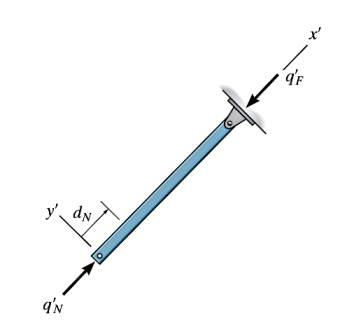
\includegraphics[width=15em]{phy_020_strs_05_06.jpg}

Makaşkiriş öğelerinin sadece eksenel yüklenebildiklerini biliyoruz, eğer üstteki
figür gibi bir senaryo olsaydı, alt uçtan $q'_N$ kuvveti uygulanmış, diğer nokta
bir pime bağlı, bu durumda önceki formülü değiştirip [4, sf. 542]

$$
\Delta = \frac{NL}{AE} \to \frac{\Delta AE}{L} = N
$$

ve $\Delta$ yerine yer değişim $d_N$, kuvvet $N$ için $q'_N$ kullanırız,

$$
q'_N = \frac{AE}{L} d_N
$$

Pimli noktada denge durumunda üstteki kuvvete tepki olarak ona eşdeğerde ama
eksi yönde bir kuvvet oluşmalıdır, ona $q'_F$ diyelim, o zaman diğer uçta

$$
q'_F = -\frac{AE}{L} d_N
$$

olur.

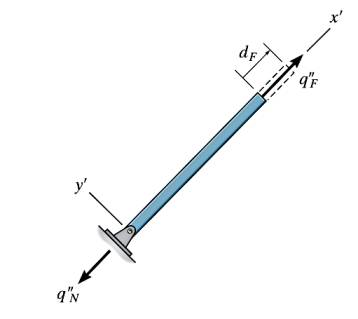
\includegraphics[width=15em]{phy_020_strs_05_07.jpg}

Eğer pimli noktayı değiştirsek, üstteki duruma baksak, o zaman yer değişim
$d_F$ içeren iki formül şöyle olur,

$$
q''_N = - \frac{AE}{L} d_F \quad
q''_F = - \frac{AE}{L} d_F 
$$

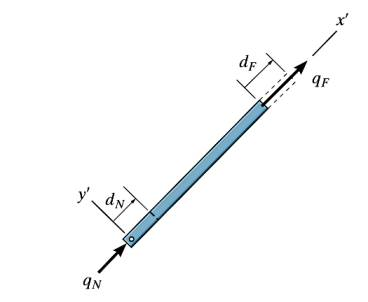
\includegraphics[width=15em]{phy_020_strs_05_08.jpg}

Gördüğümüz iki senaryo, yani bir uçta pim var diğerinde yok, sonra tam tersi,
bize dört formül verdi. Eğer her uçta pim olduğu durumu elde etmek istersek, ki
bu durum daha büyük bir makaskiriş sisteminde olurdu, o zaman bu dört formülü
üst üste koymak (superposition) gerekli,

$$
q_N = q'_N + q''_N 
$$

$$
q_F = q'_F + q''_F
$$

Yani

$$
q_N = \frac{AE}{L} d_N - \frac{AE}{L} d_F
$$

$$
q_F = -\frac{AE}{L} d_N + \frac{AE}{L} d_F
$$

Üstteki iki formülü matris formunda yazmak istersek,

$$
\left[\begin{array}{c}
q_N \\ q_F
\end{array}\right] =
\left[\begin{array}{cc}
1 & -1 \\ -1 & 1
\end{array}\right]
\left[\begin{array}{c}
d_N \\ d_F
\end{array}\right] 
$$

Daha kısa olarak

$$
q = k' d
$$

ki $q,k',d$ vektör, matris formundadır ve

$$
k' = \left[\begin{array}{cc}
1 & -1 \\ -1 & 1
\end{array}\right]
$$

$k'$ matrisine öğe direngenlik matrisi (member stiffness matrix) olarak bilinir.

Kirişler

Eksene dik (transverse) yüklerin dinamiğini hesaplamak için kiriş formülasyonu
gerekli. Bu kiriş parçasının iki ucuna bakacağız, bu uçlar yer değişimine ve
ufak bir dönüş açısına sahip olabilecekler. Yani her uçta iki olmak üzere
bu sistemde toplam dört derece serbestlik var. Fonksiyon $v(x)$,

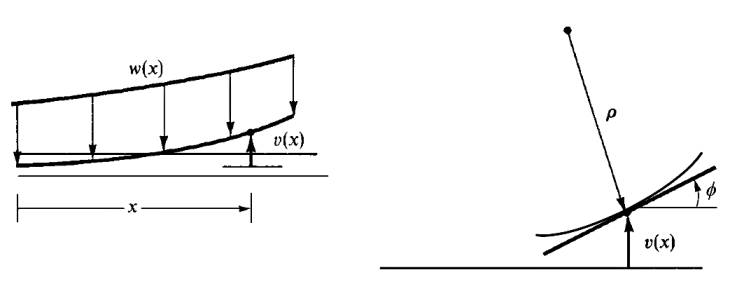
\includegraphics[width=20em]{phy_020_strs_05_09.jpg}

Bu fonksiyonu

$$
v(x) = a_1 x^3 + a_2 x^2 + a_3 x + a_4
\mlabel{7}
$$

kupsel polinom ile temsil edebiliriz, bu uygun çünkü 4 derece serbestlik var
demiştik, üstteki formülde de böyle. Ayrıca kupsel fonksiyonlar iki parça
yanyana geldiğinde eğimsel ve yer değişim sürekliliğini de sağlayabilirler.

$x=0$ ve $x=L$ noktalarında elde edilebilecek formüllere bakalım [7, sf. 173],

$$
v(0) = v_1 = a_4
$$

$$
\frac{\ud v(0)}{\ud x} = \phi_1 = a_3
$$

$$
v(L) = v_2 = a_1 L^3 + a_2 L^2 + a_3 L + a_4 
$$

$$
\frac{\ud v}{\ud x}(L) = \phi_2 = 3 a_1 L^2 + 2 a_2 L + a_3
$$

ki $\phi = \ud v / \ud x$, üstteki resimde ima edildiği gibi, ve $\phi$'nin
ufak dönüşlere tekabül ettiği durumlar için.

Üstteki dört formülü kullanarak (7) içindeki katsayılar yerine serbestlik
derecesi değişkenleri $v_1,v_2,\phi_1,\phi_2$ kullanabiliriz, biraz cebirsel
takla atmak lazım. $a_3,a_4$ için ne koyulacağı bariz, bunlar sırasıyla
$\phi_1,v_1$ olacak. Geriye $a_1,a_2$ kalıyor, bunun için $v_2,\phi_2$
formüllerini $a_1$ için düzenleyip birbirine eşitlersek, iptaller sonrası
geriye $a_2$ eşitliği ortaya çıkacaktır, benzer şekilde $a_1$ elde edilebilir,
nihai sonuç,

$$
v =
\left[
  \frac{2}{L^3} (v_1 - v_2) + \frac{1}{L^2} (\phi_1 - \phi_2) 
\right] x^3 +
\left[
  -\frac{3}{L^2} (v_1 - v_2) - \frac{1}{L} (2\phi_1 + \phi_2)
\right] x^2 +
\phi_1 x + v_1
\mlabel{8}
$$

Bu nihai formülü kullanarak kiriş öğe direngenlik matrisi elde
edilebilir. Bu matris için iki uçtaki kaykılma kuvvetleri ve
bükülme momentleri gerekiyor, onlara $f_{1y}$, $m_1$, $f_{2y}$,
$m_2$ diyelim,

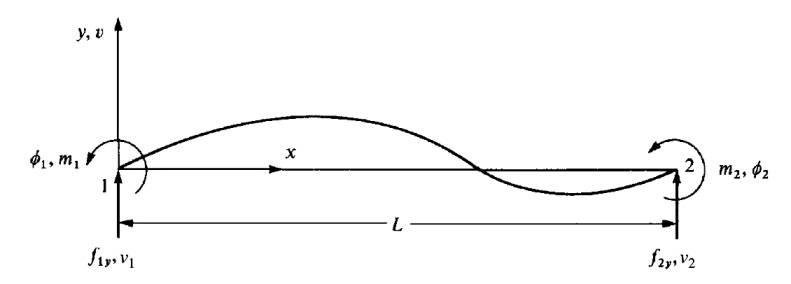
\includegraphics[width=20em]{phy_020_strs_05_10.jpg}

Moment $m(x)$, kaykılma $V$ formüllerini bir kez daha hatırlarsak

$$
m(x) = EI \frac{\ud^2 v}{\ud x^2}, \quad
V = EI \frac{\ud^3 v}{\ud x^3}
$$

Türevi alınan $v$ formülü (8)'de gösterilen olacak, o zaman

$$
f_{1y} = V = EI \frac{\ud^3 v(0)}{\ud x^3} =
\frac{EI}{L^3} (12 v_1 + 6L \phi_1 - 12 v_2 + 6L \phi_2 )
$$

$$
m_1 = -m = -EI \frac{\ud^2 v(0)}{\ud x^2} =
\frac{EI}{L^3} ( 6L v_1 + 4L^2 \phi_1 - 6L v_2 + 2 L^2 \phi_2 )
$$

$$
f_{2y} = -V = -EI \frac{\ud^3 v(L)}{\ud x^3} =
\frac{EI}{L^3} (-12 v_1 - 6L \phi_1 + 12 v_2 - 6L \phi_2 )
$$

$$
m_2 = m = EI \frac{\ud^2 v(L)}{\ud x^2} =
\frac{EI}{L^3} ( 6L v_1 + 2L^2 \phi_1 - 6L v_2 + 4 L^2 \phi_2)
$$

Matris formunda üstteki dört formülü şu şekilde gösterebiliriz,

$$
\left[\begin{array}{c}
f_{1y} \\ m_1 \\ f_{2y} \\ m_2
\end{array}\right] =
\frac{EI}{L^3}
\left[\begin{array}{cccc}
12 & 6L & -12 & 6L \\
6L & 4L^2 & -6L & -6L \\
-12 & -6L & 12 & -6L \\
6L & 2L^2 & -6L & 4L^2
\end{array}\right]
\left[\begin{array}{ccc}
v_1 \\ \phi_1 \\ v_2 \\ \phi_2
\end{array}\right]
$$

Direngenlik matrisi denen büyüklük $EI / L^3$ çarpı üstteki formülde görülen
4 x 4 matrisidir, yani eşitliğin sağında orta kısımda olan değerler.

Ornek

Daha önce makaskirişlerde gördüğümüz gibi üstdüşüm tekniğini normal kirişler
için de kullanmak mümkündür. Alttaki gibi bir yapı düşünelim [7, sf. 181],

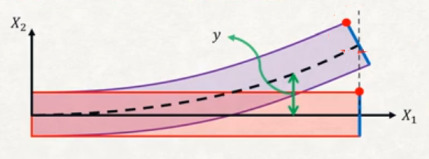
\includegraphics[width=20em]{phy_020_strs_06_01.jpg}

$EI$ büyüklüğünün tüm kiriş boyunca sabit olduğunu kabul edelim. Kirişin orta
noktasına 5000 N kuvveti ve 2500 Nm momenti uygulanıyor. Kiriş en solda bir
duvara sabitlenmiş, sağ noktasında ise bir pimle destekleniyor (pimler
dönüşe izin verir ama yer değişime izin vermez). 

Bu yapıyı üç tane düğüm (node) üzerinden ayrıksal hale getirebiliriz,
düğümler 1,2, ve 3, ve elde iki tane kiriş var, grafikte görülüyor.

Bu iki kiris parcasi icin direngenlik matrisleri,

$$
k^{(1)} = \frac{EI}{L^3}
\begin{array}{cc} & \begin{array}{rrrr} v_1 & \phi_1 & v_2 & \phi_2 \end{array} \\ &
\left[
\begin{array}{cccc}
  12 & 6L & -12 & 6L \\
  6L & 4L^2 & -6L & 2L^2 \\
  -12 & -6L & 12 & -6L \\
  6L & 2L^2 & -6L & 4L^2
\end{array}
\right]
\end{array} 
$$

$$
k^{(2)} = \frac{EI}{L^3}
\begin{array}{cc} & \begin{array}{rrrr} v_2 & \phi_2 & v_3 & \phi_3 \end{array} \\ &
\left[
\begin{array}{cccc}
  12 & 6L & -12 & 6L \\
  6L & 4L^2 & -6L & 2L^2 \\
  -12 & -6L & 12 & -6L \\
  6L & 2L^2 & -6L & 4L^2
\end{array}
\right]
\end{array} 
$$

[devam edecek]

Kaynaklar

[1] Bayramlı, {\em Fizik, Materyel Mekaniği - Hazırlık}

[2] Craig, {\em Mechanics of Materials, Third Edition}

[3] Bayramlı, {\em Çok Değişkenli Calculus, Eğrilik (Curvature)}

[4] Hibbeler, {\em Structural Analysis, 8th Edition}

[5] Bayramlı, {\em Hesapsal Bilim, Ders 1-15}

[6] Gere, {\em Mechanics of Materials}

[7] Logan, {\em A First Course in the Finite Element Method}

\end{document}


